\documentclass [12pt] {article}
\usepackage[dvips]{graphicx}
\usepackage{color}
\usepackage{amssymb,amsmath,amsfonts,amsthm,bm}
\usepackage{xfrac}
\usepackage[backref,letterpaper]{hyperref}
\usepackage{pgfplots}

\textheight 9.0in
\textwidth 6.5in
\oddsidemargin -0.225in
\evensidemargin -0.225in
\topmargin -0.5in

\newcommand{\bfdelta}{{\bm{\delta}}}
\newcommand{\bfnu}{{\bm{\nu}}}
\newcommand{\bff}{{\bm{f}}}
\newcommand{\bbC}{{\mathbb{C}}}
\newcommand{\calD}{{\mathcal{D}}}
\newcommand{\bbF}{{\mathbb{F}}}
\newcommand{\calL}{{\mathcal{L}}}
\newcommand{\bbR}{{\mathbb{R}}}
\newcommand{\bfP}{{\mathbf{P}}}
\newcommand{\calS}{{\mathcal{S}}}
\newcommand{\bfu}{{\mathbf{u}}}
\newcommand{\bfv}{{\mathbf{v}}}
\newcommand{\bfw}{{\mathbf{w}}}
\newcommand{\bfx}{{\mathbf{x}}}
\newcommand{\bfy}{{\mathbf{y}}}
\newcommand{\bfz}{{\mathbf{z}}}
\newcommand{\bbZ}{{\mathbb{Z}}}
\newcommand{\bfzero}{{\mathbf{0}}}
\newcommand{\bfone}{{\mathbf{1}}}
\newcommand{\Var}{{\mbox{Var}}}
\newcommand{\notsubseteq}{{\subseteq \hspace{-0.15in}/\;}}
\newcommand{\nin}{\notin}
\newcommand{\addlink}[2]{{\htmladdnormallink {\textcolor{blue}{{#1}}}{{#2}}}}
\newcommand{\Prob}{{\mbox{Prob}}}
\newcommand{\supp}{{\mbox{supp}}}


%%%%%%%%%%%%%%%%%%%%%%%
%
% Change course, date, etc. here and the 
% header will be automatically generated.
%
%%%%%%%%%%%%%%%%%%%%%%%

\newcommand{\class}{Math 166}
\newcommand{\classname}{Statistics}
\newcommand{\term}{Spring 2023}
\newcommand{\assignment}{Homework 9}
\newcommand{\duedate}{Due 11:59pm Apr. 2, 2023}
%%%%%%%%%%%%%%%%%%%%

\begin{document}

\thispagestyle{empty}

\noindent \textbf{\class \hfill \assignment~\footnote{\copyright 2022, Bruce M. Boghosian, edited by Merek Johnson, all rights reserved.}}\\
\textbf{\classname \hfill \duedate} \\
\rule[1ex]{\textwidth}{.1pt}
\textbf{Book problems: 10.2.2}\\
In this problem, the probability the each of the four phenotypes would be selected from four trials is a multinomial distribution. Plugging in the provided values:
\begin{align*}
\frac{n!}{k_1!k_2!... k_t!}p_1^kp_2^k...p_t^k
&= \frac{4!}{1!1!1!1!}\left(\frac{9}{16}\right)^1\left(\frac{3}{16}\right)^1\left(\frac{3}{16}\right)^1\left(\frac{1}{16}\right)^1\\
&\approx 0.02966
\end{align*}
\\
\textbf{Book problems: 10.2.10}\\
\\
\textbf{Written problems: 1a}\\
If the sample was indeed from a uniform distribution on [0,1], each of the four equal-length intervals would contain 5 observations. Based on the sample, the distribution looks like:\\
\\
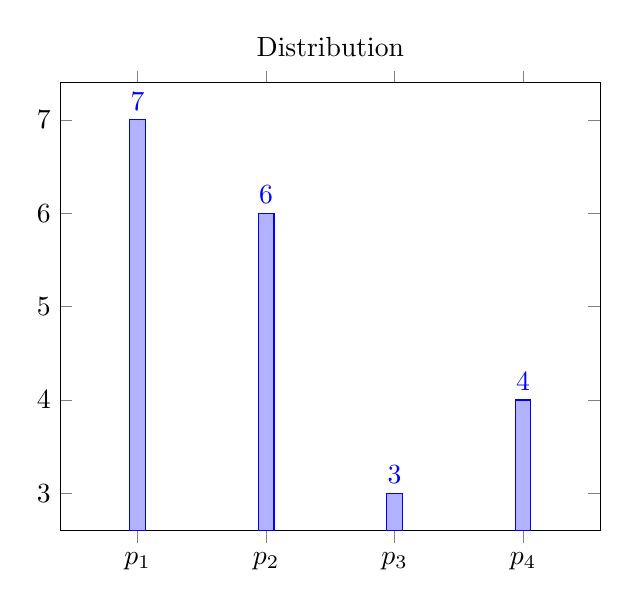
\begin{tikzpicture}
\begin{axis}
[
title=Distribution,
ybar,
nodes near coords,bar width=0.2cm,
symbolic x coords={$p_1$,$p_2$,$p_3$,$p_4$},
enlarge x limits = .2,
]
\addplot coordinates {($p_1$,7) ($p_2$,6) ($p_3$,3) ($p_4$,4)};
\end{axis}
\end{tikzpicture}
\\	
The hypothesis test for this is $H_0: p_1 = p_2 = p_3 = P_4$ and $H_1: p_i \neq p_i$ for at least one $i$. If $d \geq \chi_{1-\alpha,t-1}^2$, we will reject the null hypohtesis. We can calculate $d$ as:
\begin{align*}
d
&= \sum_{i=1}^t\frac{(k_i-np_i)^2}{np_i}\\
&= \frac{(7-5)^2}{5}+\frac{(6-5)^2}{5}+\frac{(3-5)^2}{5}+\frac{(4-5)^2}{5}\\
&= 2
\end{align*}
Assuming $\alpha = 0.05$, the test statistic for $\chi_{0.95,19}^2 =  7.815$. Given 2 $\geq$ 7.815, we fail to reject the null hypothesis. There is not evidence against this assumption.\\
\\
\textbf{Written problems: 1b}\\
We can conduct a similar test, this time to assess whether the sample was from a uniform distribution $[0,2]$.

\begin{enumerate}

\item The following sample of $n=20$ is supposedly generated from a random number generator using uniform distribution on the interval $[0,1]$:
\[
\{.11, .56, .72, .18, .26, .32, .42, .22, .96, .04, .45, .22, .08, .65, .32, .88, .76, .32, .21, .8\}
\]

\begin{enumerate}
    \item After grouping the data using a partition of four equal-length intervals, perform the appropriate hypothesis test to assess whether there is evidence against this assumption.
    \item Suppose we have the same sample but the claim is that it came from a uniform distribution on the interval $[0,2]$. Perform another hypothesis test and argue that the conclusion agrees with our intuition based on the values in the given sample.
\end{enumerate} 

\item Suppose you want to run a goodness-of-fit test on a sample to determine whether the data came from some hypothesized continuous pdf $f_0(y)$ (where all parameters are known). You get a sample $\{Y_1, Y_2, \ldots, Y_n\}$ and group your outcomes into $t$ outcome buckets $r_1, r_2, \ldots, r_t$ with sizes $X_1, X_2, \ldots, X_t$, respectively. You obtain the $\chi^2$ statistic $d$ with $t-1$ degrees of freedom, which has a corresponding p-value $P$. 

Now imagine you obtain a new sample which consists of exactly two copies of all the data from the first sample, that is $\{Y_1, Y_1, Y_2, Y_2, \ldots, Y_n, Y_n\}$. Using the same buckets from your initial sample, for this data you will get a different statistic $d^*$ (also with $t-1)$ degrees of freedom and p-value $P^*$.

\begin{enumerate}
    \item Find $d^*$ as a function of $d$
    \item Will $P^*$ be larger or smaller than $P$?
    \item Compare the two p-values. Does the difference agree with your intuition? 
\end{enumerate}

\end{enumerate}

\end{document}
